\documentclass{article}[jsarticle]
\usepackage[T1]{fontenc}
\usepackage[dvipdfmx]{hyperref}
\usepackage{lmodern}
\usepackage{latexsym}
\usepackage{amsfonts}
\usepackage{amssymb}
\usepackage{mathtools}
\usepackage{nccmath}
\usepackage{amsthm}
\usepackage{multirow}
\usepackage{graphicx}
\usepackage[dvipdfmx]{color}
\usepackage{wrapfig}
\usepackage{here}
\usepackage{float}
\usepackage{ascmac}
\usepackage{url}
\usepackage{caption}

% Generated by ChatGPT
\usepackage{listings}
\usepackage{xcolor}

\lstset{
    basicstyle=\ttfamily\color{white},
    numbers=none,  % Line numbers
    numberstyle=\tiny\color{white},
    numbersep=5pt,
    tabsize=2,
    extendedchars=true,
    breaklines=true,
    keywordstyle=\color[rgb]{0.58,0.00,0.83},
    stringstyle=\color[rgb]{0.81,0.36,0.00},
    identifierstyle=\color{white},
    commentstyle=\color[rgb]{0.34,0.62,0.16},
    rulecolor=\color[rgb]{0.5,0.5,0.5},
    xleftmargin=0.1cm,    % Left margin
    xrightmargin=0.1cm,   % Right margin
    language=python,
    backgroundcolor=\color[rgb]{0.13,0.13,0.13},
    showspaces=false,
    showstringspaces=false
}



\title{2023年度 特別研究2 研究状況報告書}
\author{高林秀 \\ 三宅研究室 博士前期課程1年 \\ V-CampusID : 23vr008n}
\date{\today}

\begin{document}

\maketitle

\begin{abstract}
    本稿は本年度特別研究2の研究状況報告を記載するものである.\par
    本稿の構成は,第一章において研究計画の概要,第二章において研究計画が確定した昨年度7月から本年1月までに行った研究活動について,
    第三章において現在の研究の進捗状況と課題点について,第四章において来年度特別研究3以降の修士論文までの計画を示す.\par 
    %TODO:第一章の概要
    %TODO:第二章の概要
    %TODO:第三章の概要
    %TODO:第四章の概要
    なお巻末には参考文献と,本稿記載の実験環境を格納したリポジトリのURLを記載する.
\end{abstract}



\tableofcontents


\section{研究計画の概要}
本章では,昨年の特別研究1で提出した研究計画について,研究テーマ,研究背景,本研究が目指す目標について簡単に記載する.
\subsection{研究テーマ}
    \centerline{
        \textbf{マルチエージェント強化学習を利用した,} \\
        \textbf{自律型ドローンによる災害対応アプローチ}
    }
    大規模災害時の被災者救助や救援物資輸送の効率化,省人化を目指す.
    具体的には,ドローンとマルチエージェント強化学習を組み合わせた新たなアプローチを開発し,その有効性を検証する.
\subsection{研究背景}
\paragraph{自衛隊員の不足} \par 
災害大国である我が国において,被災者の捜索,被害状況の把握,
救援物資の現地輸送といった対応は,迅速かつ効率的に行われなければならない.しかし近年,そのような災害対応を一任務とする,
自衛隊員の人材が不足している,あるいは今後さらに不足する事態が予想されている.\par 
以下は\href{http://www.clearing.mod.go.jp/hakusho_data/2022/html/ns056000.html}{令和4年版 防衛白書の自衛官の定員及び現員並びに自衛官の定数と現員数の推移に関する資料}である.
\begin{figure}[H]
    \centering
    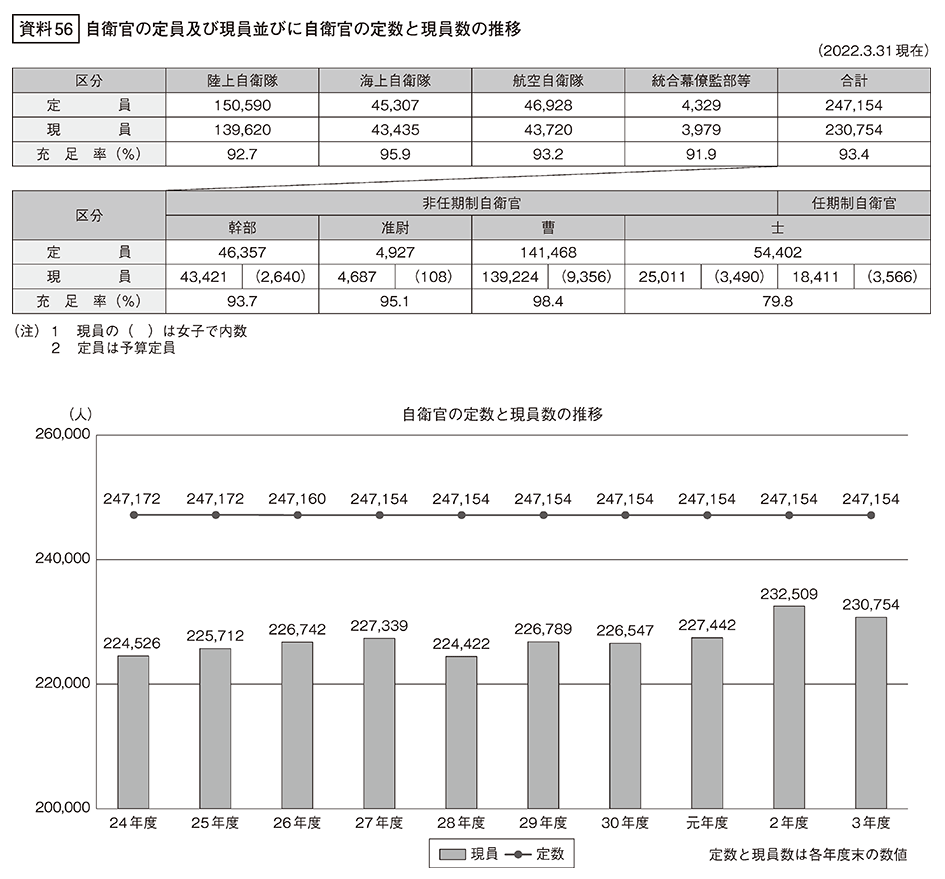
\includegraphics[scale=0.3]{./Images/20240203195052.png}
    \caption{自衛官の定員及び現員並びに自衛官の定数と現員数の推移}
\end{figure}
このように,平成24年度からの統計でも,自衛官の定員数と現員数には$16000$名前後の開きがあり,法律で定められた定員を満たせていない.\par
採用の観点では,2022年度の任期制自衛官の採用で、候補生が計画数の4割ほどしか集まらず、過去最低となった事例がある\cite{news01}.
今後の,少子高齢化が進む我が国において,自衛隊員の不足は深刻な問題となることが予想されている.

\paragraph{陸上自衛隊におけるドローン配備の増強と活用}
防衛省は2020年に,同年末までに陸上自衛隊のドローン配備数を合計201機とすることを発表\cite{news02}していた.
2018年末の時点での配備数は計で13機であったため,大幅な増強をおこなうこととなった.\par
このドローン増強の背景として,2018年9月に発生した北海道胆振東部地震がある.人が入り込めない山奥や広いエリアを短時間で撮影できる利点が評価され,導入が進められた.\par
2019年の防衛白書では,人員の進入困難な箇所や方向から地上部隊がドローンを飛ばし,救助を待つ人がどこにいるかなどの情報を迅速に提供したと明記され,陸上自衛隊の各基地にドローンを1,2機ずつ配備する体制が進んでいた.\par
また,同年2月には,陸上自衛隊東部方面総監部とJUIDA(日本UAS産業振興協議会)\footnote{一般社団法人日本UAS産業振興協議会 JUIDA:我が国における無人航空機no
の産業振興を目的に2014年7月に設立された.無人航空機の情報周知活動や,航行ガイドラインの策定,市場創造支援などに取り組んでいる.}が大規模災害発生時における相互協力を目的とした協定を締結しており,今後自衛隊の災害派遣においてドローンの利活用がさらに進むことが予想される.
\paragraph{レベル4飛行の解禁} \par
レベル4飛行とは,有人地帯での目視外飛行のこと.目視で監視できない状態で,有人地帯上空を自律飛行することができる飛行レベルを指す.
我が国では2022年12月5日に改正航空法が施行され,レベル4飛行が解禁された\cite{doc01}.\par 
これにより,現在ドローンの災害対応における有効性に注目が集まっている.

\subsection{本研究の方向性}
本研究は,強化学習モデルとドローンの災害対応における有効性を示す,工学的な研究として進める.
具体的には,以下のような方向性で研究を進める.
\begin{itemize}
    \item 強化学習を活かせる部分とそうでない部分を調査
    \item 災害対応において強化学習を活かせる部分(自明でなくルールベースでできない部分)を調査し,問題設定を行う.
    \item 上記の問題に対して,強化学習を用いた解法が有効であることを示す.
\end{itemize}

\subsection{本研究が目指す目標}
本研究では,災害で孤立した街や都市を再現し,複数のドローンをエージェントとした強化学習に
よって,被災者の捜索,救援物資の輸送の最適化を模索し,自律型ドローンの災害時における有用性を検証する. 
また,学習したモデルを用いて,実際のドローンを用いた飛行までの技術開発と飛行実験まで行うことを目標とする.


\section{研究活動報告}
本章では昨年度7月の研究計画の確定から本年1月までに行った研究活動について記載する.
\subsection{災害対応における問題点の調査}
まず,本研究の目標の一つである災害時における物資輸送について,過去の大規模災害時の事例を元に調査を行った.
\subsubsection{災害時の物資輸送フロー}
まず,災害時の物資輸送フローについて調査を行った.以下は, 平成23年に国土交通省が作成した,『救援物資物流システムの基本的な考え方に関するアドバイザリー会議』\cite{doc02}の報告書から要約し,まとめたものである.
この報告書には,災害時における救援物資の基本的な輸送フローについてまとめられており,物資の発送から各避難所への到着までの流れが記載されている.
\begin{figure}[H]
    \centering
    
\includegraphics[width=\textwidth]{./Images/20240127180600.png}
    \caption{救援物資輸送の基本フロー}
\end{figure}
一次物資集積拠点では,救援物資を荷下ろしし,市町村毎の二次物資集積拠点毎に救援物資を仕分けし,トラック等の輸送手段に積み替え,救援物資は二次物資集積拠点に輸送される.
二次物資集積拠点では,一次物資集積拠点から輸送された救援物資を荷下ろしし,今度は避難所毎に救援物資を仕分けし,さらにトラック等の輸送手段に積み替え,救援物資は避難所に輸送され,最終的に被災者の下に救援物資が届けられることになる.発地から直接二次物資集積拠点や避難所まで直接輸送される救援物資もある.\par 

\subsubsection{災害時の物資輸送における問題事例調査}
次に,大規模災害時実際に救援物資輸送に際し,どのような問題が発生したのかを調査した.ここでは,その一部として研究ミーティングでも報告した,阪神淡路大震災と東日本大震災における事例を示す.
\paragraph{1995年 阪神淡路大震災} 
以下は,内閣府防災情報に掲載されている『阪神淡路大震災教訓情報資料集~第1期初動対応\cite{doc03}』からの抜粋である.この資料集には,阪神淡路大震災において,救援物資輸送の際に遭遇した問題点がまとめられている.\par
道路の寸断,交通集中による渋滞などにより,輸送が滞るという事態が報告されている.
\begin{quote}
    地震発生翌日から,被災地域に急行する緊急物資等輸送車両や救援車両が渋滞のため立ち往生したり,遠方からの緊急物資等輸送車両が指定された目的地がわからず右往左往する状況があり,それに応するため,交通機動隊の白バイとパトカーにより救助・救援車両等の先導・誘導活動を実施した.\par 
    \ldots \par
    阪神高速道路の倒壊により東西を結ぶ代替道路が激しく渋滞し,物資の輸送には非常に多くの時間がかかった.\par 
    \ldots \par
    翌日になっても渋滞は物資の輸送を妨げた.午前10時に連絡を受けて,王子陸上競技場に空輸された物資を受け取りにいった車は,5キロを2往復するのに8時間かかった
\end{quote}
このように,幹線道路の寸断や道路設備破壊による交通の混乱により,救援物資の輸送に時間がかかったという事例が報告されている.現地に集積まではできたとしても,その後の受け取りから配送において多くの時間がかかってしまったという事例だ. \par 
また,空路においても問題が発生している.
\begin{quote}
    ヘリコプターは緊急物資や医師団の輸送に大きな力を発揮した.しかし,ポートアイランドに設けられた肝心のヘリポートが滑走路のひび割れなどで,その機能は低下していた.\par
    \ldots \par
    臨時のヘリポートを開設した.それでも,誘導標識がないなど,設備面はもとより,全体としてヘリポートの量的な不足は否めなかった.
\end{quote}
陸路に加えて,空路での輸送も実施はされたが,ヘリポートへの被害や,その数自体が不足するなどの課題も浮彫となった.

\paragraph{2011年 東日本大震災}
被災地域の自治体では,指揮系統の混乱や人員不足,機能不全による救援物資輸送の課題が報告されている.以下は,東北大学が掲載している『南三陸町 東日本大震災 職員初動対応等検証 報告書\cite{doc04}』からの抜粋である.
\begin{quote}
    物資の避難所への配送には,町職員では人員が足らないことから,運送業者や自衛隊,町民にもお願いをして対応した.\par 
    \ldots \par
    第一に,町職員が物資の仕分け・管理・配送をするのは限界があるにもかかわらず,物資管理の専門の宅配業者から支援を受けるのに時間がかかったことである.\par 
    \ldots \par
    第二に,燃料は先に調達体制ができたが,受入れ体制が整うまでに時間がかかってしまい,数日程度供給が滞ってしまったことである.\par
    \ldots \par
    第三に,ベイサイドアリーナは,トラックが 1 台ずつしか通れず,入り口にトランシーバーを持った職員を配置して運用しないといけない構造で,人員が必要でかつ時間がかかったことである.
\end{quote}
このように南三陸町の事例では,人手不足による要因と,被災後の行政の機能不全による救援物資輸送の問題点が挙げられていた.
\paragraph{まとめ}
以上の事例から,災害時における救援物資輸送において,以下のような問題点があることがわかった.
\begin{itemize}
    \item 道路の寸断や交通集中による渋滞により,救援物資の輸送に時間がかかる.
    \item 空路においても,ヘリポート/航空設備の被害や,数の不足により,迅速に救援物資の輸送を行えない.
    \item 人手不足により,救援物資の輸送体制が整わず,被災者への救援物資の供給が滞る.
    \item 行政の機能不全と指揮系統の混乱により,迅速な救援物資の輸送が行えない.
\end{itemize}

\subsection{ドローンの災害時活用事例時事調査}
ドローンの災害時における活用,研究事例を調査した.この章では,過去の我が国における災害時において,実際にドローンが活用された事例を2つ示す.
\paragraph{全国初のドローンによる救援物資の輸送事例}
これは,大分県,佐賀県,福岡県において2023年6月末から同年7月16日にかけて降り続いた大雨に関する事例である.
この大雨では,6月28日から7月16日までの総降水量が大分県,佐賀県,福岡県で$1,200$ミリを超え,気象庁は7月10日朝に福岡県と大分県を対象に大雨特別警報を発表する事態にまで発展した.\par
この大雨で大分県の由布市では,地滑りが発生し,住宅1棟が倒壊,住民2人が孤立するという状況があった.\par 
発生直後,防災ヘリコプターを飛ばせなかったことから,食料や水,救助隊と連絡を取り合う衛星電話などの救援物資を届けるためにドローンを使った全国初の事例となった.\par 
大分県によれば,物資を配送する拠点から孤立した住宅まで,徒歩だとおよそ2時間かかるところが3分で輸送できたという.\par
この事例では,ドローンによる救援物資の輸送が実際に行われ,土砂災害で孤立した地域に対して,ピンポイントかつ迅速に救援物資の輸送ができた事が示された.
また,この大雨で発生した土砂崩れや河川の氾濫の被害状況の調査でも活用されたという.\cite{news03}
\paragraph{令和6年度 能登半島地震における事例}
本年初頭に発生した能登半島地震においても,官民連携でドローンが活用された事例がある.\par 
本年1月8日,石川県輪島市において孤立地域・世帯に対しドローンによる薬の輸送が行われた.700人以上が孤立状態になっている輪島市鵠巣地区に向けて市内の中心部から薬を配送した\cite{news04}.
JUIDA(日本UAS産業振興協議会)は,能登半島地震の発生後,輪島市から要請を受けてドローンを使った捜索や物資の輸送を行っている.\par 
また,本地震の事例では救援物資の輸送以外にも,被害状況の偵察と物資運搬ルート探索においてドローンが活用された.
株式会社SkyDrive\footnote{株式会社SkyDrive:電動垂直離着陸型無操縦者航空機(eVTOL)の研究開発,製造販売を行っている愛知県豊田市挙母町に本社を置くメーカー.物流ドローンの開発・製造・販売・運用サービス・コンサルティング等も行っている.}は,陸上自衛隊 豊川駐屯地の第十特科連隊からの要請に基づき,本年1月8日から14日まで,石川県輪島市において被害状況の確認および救援物資の輸送のルート探索で,ドローンを活用した\cite{news05}.
\begin{figure}[H]
    \centering
    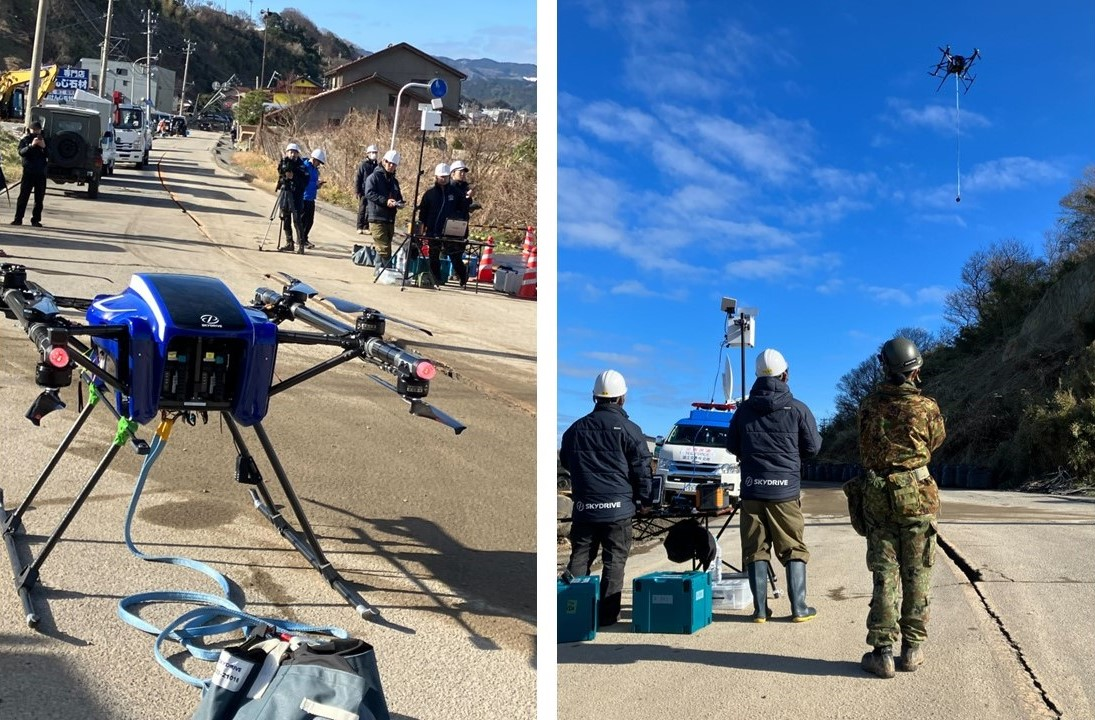
\includegraphics[scale=0.2]{./Images/202401311838.jpg}
    \captionsetup{justification=centering}
    \caption{
        SkyDrive社によるドローン支援の様子 \\
        出典: \url{https://www.skydrive2020.com/news/20210115/}
    }
\end{figure}

\subsection{ドローンの性能調査と法的制約}
この章では,ドローンの性能(連続飛行可能時間,最大積載量)と我が国での運用における法的制約について調査した.
\subsubsection{ドローンの分類と性能}
\paragraph{ドローンの法的分類}
ドローンには,機体重量により法律上以下のように分類されている.
\begin{itemize}
    \item 200g未満:小型無人機
    \item 200g以上:無人航空機
\end{itemize}
この2つの分類に基づいて,ドローンの運用における法的制約が定められている.以下は,首相官邸が公表している資料である.
\begin{figure}[H]
    \centering
    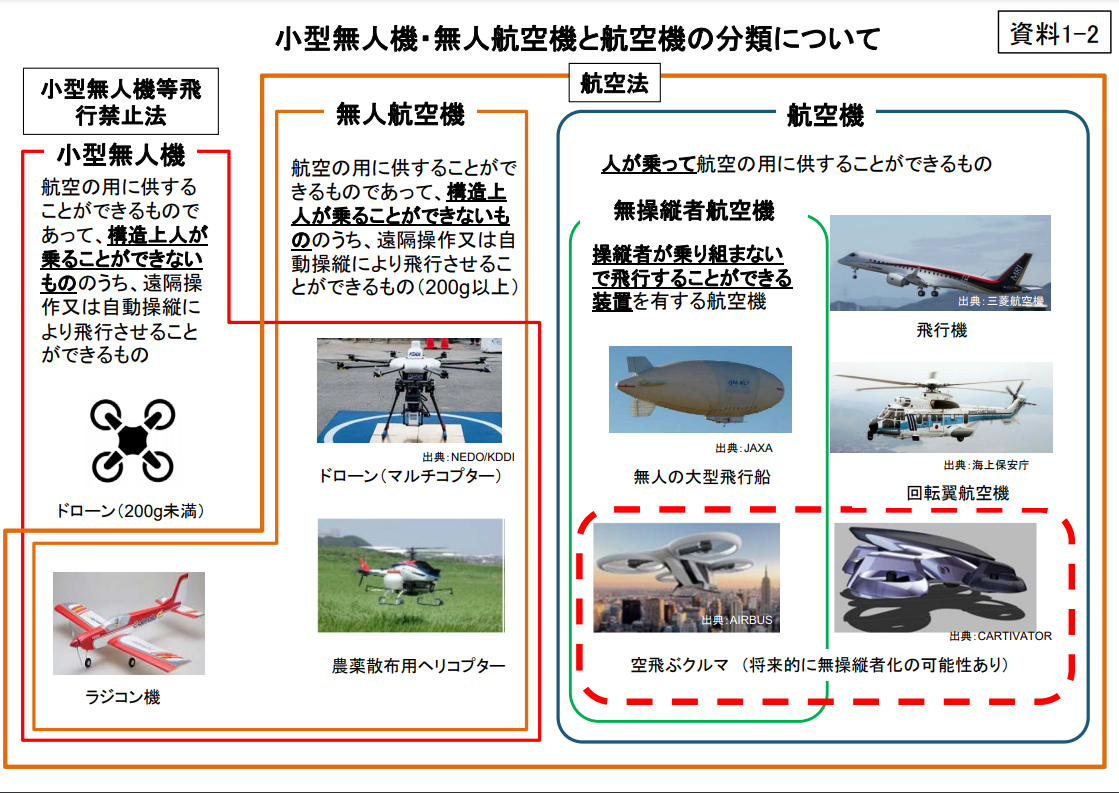
\includegraphics[width=\textwidth]{./Images/20240203205430.png}
    \captionsetup{justification=centering}
    \caption{
        小型無人機・無人航空機と航空機の分類について \\
        出典: \url{https://www.kantei.go.jp/jp/singi/kogatamujinki/kanminkyougi_dai8/s1-2.pdf}
    }
\end{figure}
\subsubsection{ドローン運用の法的制約}
我が国では,ドローンの運用については航空法と小型無人等飛行禁止法により定められている事項がある.以下はその主な制限事項である.
\begin{itemize}
    \item 飛行禁止空域に関する取り決め
    \begin{itemize}
        \item 空港周辺での飛行の禁止
        \item 人口密集地での飛行の禁止
        \item 高度$150m$以上での飛行の禁止
        \item 緊急用無空域\footnote{}での飛行の禁止
    \end{itemize}
    \item 飛行方法に関する取り決め
    \begin{itemize}
        \item アルコール又は薬物等の影響下で飛行させないこと
        \item 航空機又は他の無人航空機との衝突を予防するよう飛行させること
        \item 他人に迷惑を及ぼすような方法で飛行させないこと
        \item 飛行前に安全確認を行うこと 
    \end{itemize}
\end{itemize}
また,以下の飛行方法に関しては,一等無人航空機操縦士などの資格を有する者が,あらかじめ地方航空局長の承認を受けることが定められている.
\begin{itemize}
    \item 夜間での飛行
    \item 目視外での飛行
    \item 人又は物件との距離を確保できない飛行
    \item 催し場所上空での飛行
    \item 危険物の輸送
    \item 物件の投下
\end{itemize}
ただし,これらの制限事項は,災害などの緊急時において国や自治体からの要請と承認を受けている場合に限り,適用されないことになっている.
以下は,国土交通省が公表している『捜索又は救助のための特例について』からの抜粋である.
\begin{quote}
    飛行禁止空域及び承認が必要となる方法における飛行については,事故や災害時に,国や地方公共団体,また,これらの者の依頼を受けた者が捜索又は救助を行うために無人航空機を飛行させる場合については,適用されないこととなっています.
\end{quote}
従って,航空法改正によりレベル4飛行(有人地帯での目視外飛行)が解禁されたとしても,その飛行には平時,災害時問わず,国や自治体からの要請と承認が必要となることになる.

\subsection{実験報告}
\subsubsection{シングルエージェントでの簡単な物資輸送シミュレーション}
\subsubsection{強化学習モデルと実機ドローンの連携を行うための技術調査}
\paragraph{PLATEAU環境と現実のデバイスとの連携}
\paragraph{ドローンの遠隔操作方法}


\section{研究の進捗状況}
本章では,昨年の特別研究1で示した計画表を元に,本年2月現在における研究の進捗状況の開示と,直面している課題点について記載する.
\subsection{現在までの進捗状況}
2章の研究活動報告で示した通り,基本的な事例の調査,ゲームエンジン上でのドローンのシミュレーション実験,強化学習モデルと実機ドローンの連携に向けた技術調査を行ってきた.
全体の進捗としては,以下の図で示す特別研究1で示した計画よりも\textbf{大幅に遅れて進行している状況}である.
\begin{figure}[H]
    \centering
    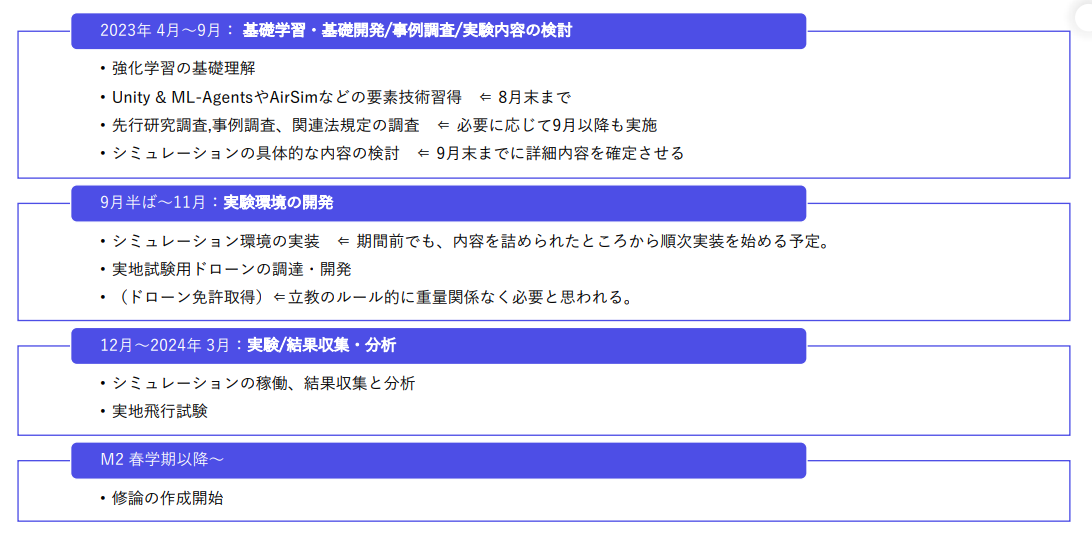
\includegraphics[width=\textwidth]{./Images/20240203171846.png}
    \captionsetup{justification=centering}
    \caption{研究計画策定当初の研究スケジュール}
\end{figure}
現段階としては,上の計画表で示した\textbf{「実験環境の開発」と,具体的な問題定義,シミュレーション内容の策定に取り掛かっている状況}である.
\paragraph{基礎学習・事例調査について}こちらは予定通りに進行した.
研究計画を策定した段階で,UnityやMLAgents,PLATEAUでのゲーム開発を通じ技術学習を行った.
事例調査については,2章で示したとおり,おもに官公庁の報告書や新聞記事を参考に行った.\par 
\paragraph{シミュレーションの内容具体化,実機ドローンでの飛行試験}
こちらは予定よりも大幅に遅れて進行している.当初の計画では昨年度11月までに,具体的な研究・シミュレーション内容を決定するはずであった.
技術学習と,基礎実験を兼ねて行っていたシングルエージェントでの実験が,2章での報告の通り,良い結果を得ることができず,こちらに時間を割いてしまい,計画通りに進行できなかった.\par 
実機でのドローン飛行試験については,その実現方法について2章で示した報告の通り,暫定ではあるものの,システムの大枠とある程度の技術選定はできている.
しかし,ドローンとモデル間の入力,出力に関していくつか課題があり,現在はそれらの解決策を模索している段階である.\par 
この点については,既にドローン5機体の購入申請を行っており,実際に開発を進めながら,解決策を見つけていく方針である.\par 
なお,実験場所として想定している立教大学構内におけるルールの確認と,本研究科事務室への確認は完了している.

\subsection{今後取り組むべき事項}
現在までの進捗状況を踏まえ,今後取り組むべき事項を以下に示す.
\begin{itemize}
    \item シミュレーションの問題設定と内容具体化
    \item 実機ドローンと強化学習モデルの連携開発
\end{itemize}
\paragraph{シミュレーションの問題設定と内容具体化}
本研究は,強化学習モデルとドローンの災害対応における有効性を示すため,災害対応における問題設定を行い,シミュレーションをもってその有効性を示すことが目標である.
しかし,現時点までその具体的な問題設定ができていないため,まずはこれを早急に確定する必要がある.\par 
考えていた問題設定の1つとして,2章での報告の通り,災害時における物資輸送の最適化/自動化を模索することに重きを置いていた.ドローンをエージェントとし,飛行制御から避難所の探索,物資輸送までを自動で行うことを目指していた.\par
しかし,強化学習は自明でないルールベースで対応できない部分に対して有効であるという点を踏まえると,強化学習を利用する部分と利用しない部分を分別すべきであり,問題設定を見直す必要がある.
特に,飛行制御や物資の取得,運搬に関しては,ルールベースで対応できる部分が多いと考えられ,あえて強化学習で対応する必要があるのか,検討する必要がある.\par
既存研究のさらなる調査と,災害対応において強化学習を活かせる部分を模索し,問題設定を行うことが現時点の喫緊の課題である.\par
現時点で強化学習を用いるべき災害対応タスクについては,以下のようなものを考えている.
\begin{itemize}
    \item 孤立地域の探索(被害状況の偵察)
    \item 各種ドローンの配置ナビゲーション
\end{itemize}
これらのタスクは,災害現場において自明ではなく,人間が上空から航空機で偵察,指示することが多いタスクであり,強化学習を用いることが有効な可能性がある.\par
\paragraph{実機ドローンと強化学習モデルの連携開発}
2章での報告の通り,実機ドローンと強化学習モデルの連携について,その実現方法の大枠は定まった.2章で示した通り,実現にあたっていくつか懸念事項,課題がある.\par
今後,購入申請したドローンが到着次第,実際に開発を進めていく予定である.そのうえで,課題の解決とさらなる課題の発見を行っていく予定である.\par 


\section{今後の研究計画}
本章では,前章の進捗状況を踏まえ,本年度 特別研究3の研究計画について記載する.\par 
初めに,改めて現在の進捗状況を整理する.
\begin{itemize}
    \item 基礎学習・事例調査については完了.ただし,これらは今後も随時継続して行う.
    \item 問題設定,シミュレーションの内容具体化,実機ドローンでの飛行試験については,大幅に遅れていて,目下進行中.
    \begin{itemize}
        \item 実機飛行試験の実現方法について,暫定ではあるものの,システムの大枠とある程度の技術選定は完了.
        \item 研究予算にてドローン5機体の購入申請済み.
    \end{itemize}
\end{itemize}
以上を踏まえて,来年度特別研究3での研究計画を以下に示す.
\paragraph{2024年 2月~3月}
\begin{itemize}
    \item マルチエージェントでの簡単な物資輸送タスクのシミュレーション開発
    \item マルチエージェント強化学習が災害対応において有効なタスクの調査
    \item 問題設定とシミュレーション内容の具体化
\end{itemize}
\paragraph{2024年 4月~5月}
\begin{itemize}
    \item モデル開発用シミュレーションの開発
    \item モデルの開発
    \item 実機ドローンのプログラム制御飛行試験
    \begin{itemize}
        \item 強化学習モデルとの連携に関連する課題の洗い出し
        \item 解決のための技術調査,開発
    \end{itemize}
\end{itemize}
\paragraph{2024年 6月~7月}
\begin{itemize}
    \item 強化学習モデルと実機ドローンの連携開発
    \item 実機ドローンでの飛行試験
    \item データの収集,分析,修論準備
\end{itemize}

\appendix
\section{制作物}
\begin{itemize}
    \item \href{https://github.com/tsyu12345/Learning-MasterPJ_BaseTech}{基礎開発用リポジトリ}
    \begin{itemize}
        \item \url{https://github.com/tsyu12345/Learning-MasterPJ_BaseTech}
    \end{itemize}
    \item \href{https://github.com/tsyu12345/PJ-PLATEAU_Award}{PLATEAU技術学習制作物}
    \begin{itemize}
        \item \url{https://github.com/tsyu12345/PJ-PLATEAU_Award}
    \end{itemize}
\end{itemize}
\section{参考}
\begin{thebibliography}{99}
    \bibitem{news01} 宮崎亜巳、Linda Sieg 田巻一彦 田中志保, 焦点:自衛隊に迫る「静かな有事」、少子化で採用難, ロイター通信, 2018年.
    \begin{itemize}
        \item \url{https://jp.reuters.com/article/idUSKCN1LZ19W/}
    \end{itemize}
    \bibitem{news02} 防衛省、自衛隊のドローン配備拡充 今年度末201機体制、災害救助に活用, 日刊工業新聞, 2019年
    \begin{itemize}
        \item \url{https://www.nikkan.co.jp/articles/view/00558763}
    \end{itemize}
    \bibitem{doc01} 航空法等の一部を改正する法律案を閣議決定, 国土交通省, 2021年
    \begin{itemize}
        \item \url{https://www.mlit.go.jp/report/press/kouku01_hh_000110.html}
    \end{itemize}
    \bibitem{doc02} 支援物資物流システムの基本的な考え方, 国土交通省, 2011年
    \begin{itemize}
        \item \url{https://www.mlit.go.jp/common/000184634.pdf}
    \end{itemize}
    \bibitem{doc03} 阪神・淡路大震災教訓情報資料集, 内閣府
    \begin{itemize}
        \item \url{https://www.bousai.go.jp/kyoiku/kyokun/hanshin_awaji/data/detail/pdf/1-7-2.pdf}
    \end{itemize}
    \bibitem{doc04} 南三陸町 東日本大震災職員初動対応等検証報告書, 南三陸町/東北大学 災害科学国際研究所, 2019年
    \begin{itemize}
        \item \url{https://www.town.minamisanriku.miyagi.jp/index.cfm/6,22334,c,html/22334/20191128-200534.pdf}
    \end{itemize}
    \bibitem{news03} 地滑りで孤立の住民に県が全国で初めてドローンで救援物資輸送, NHK, 2023s年
    \begin{itemize}
        \item \url{https://www3.nhk.or.jp/lnews/oita/20230719/5070016389.html}
    \end{itemize}
    \bibitem{news04} 地震で孤立した地域にドローンで薬を配送 石川 輪島, NHK, 2024年
    \begin{itemize}
        \item \url{https://www3.nhk.or.jp/news/html/20240109/k10014314231000.html}
    \end{itemize}
    \bibitem{news05} 能登半島地震・被災地でのドローンを活用した偵察および物資運搬のお知らせ, SkyDrive, 2024年
    \begin{itemize}
        \item \url{https://skydrive2020.com/archives/41713}
    \end{itemize}
\end{thebibliography}
\end{document}